% Builds every figure and table of the paper into a single PDF.
% make-plots.sh copies this file, plot-styles.tex, charts/, tables/ and the results into a
% build directory and runs pdflatex there.
%
% The counters are set so that each float gets the number it has in the paper: the texts
% table is Table 2, the factorization chart is Figure 3 and the (de)compression chart is
% Figure 4. Nothing in charts/ or tables/ is modified for this.
\documentclass[letterpaper,10pt,twocolumn]{article}
\usepackage[letterpaper,margin=0.9in]{geometry}
\usepackage[T1]{fontenc}
\usepackage{amsmath}
\usepackage{amssymb}

% Colours, plot styles and annotation macros used by charts/*.tex and tables/*.tex.
% Taken verbatim from the paper source (definitions.tex). Include this file if you want
% to use one of the charts in a document of your own.

\usepackage{pgfplots}
\usepgfplotslibrary{groupplots}
\usepackage{tikz}
\usepackage{subcaption}
\usepackage{xspace}

\definecolor{my-dark-red}{RGB}{183, 28, 28}
\definecolor{my-red}{RGB}{244,67,54}
\definecolor{my-pink}{RGB}{233,30,99}
\definecolor{my-purple}{RGB}{156,39,176}
\definecolor{my-deep-purple}{RGB}{103,58,183}
\definecolor{my-indigo}{RGB}{63,81,181}
\definecolor{my-blue}{RGB}{33,150,243}
\definecolor{my-light-blue}{RGB}{3,169,244}
\definecolor{my-cyan}{RGB}{0,188,212}
\definecolor{my-teal}{RGB}{0,150,136}
\definecolor{my-green}{RGB}{76,175,80}
\definecolor{my-light-green}{RGB}{139,195,74}
\definecolor{my-lime}{RGB}{205,220,57}
\definecolor{my-yellow}{RGB}{255,235,59}
\definecolor{my-amber}{RGB}{255,193,7}
\definecolor{my-orange}{RGB}{255,152,0}
\definecolor{my-deep-orange}{RGB}{255,87,34}
\definecolor{my-brown}{RGB}{121,85,72}
\definecolor{my-grey}{RGB}{120,120,120}
\definecolor{my-blue-grey}{RGB}{96,125,139}
\definecolor{my-lipics-grey}{rgb}{0.6,0.6,0.61}

\tikzset{
  empty/.style={mark=x,every mark/.append style={mark size=0.0pt}},
  3_aprx/.style={mark=diamond*,my-green,semithick,draw=black,every mark/.append style={mark size=3.2pt}},
  exact/.style={mark=square*,my-blue,semithick,draw=black,every mark/.append style={mark size=2.5pt}},
  exact_smpl/.style={mark=*,my-yellow,semithick,draw=black,every mark/.append style={mark size=2.5pt}},
  lpf/.style={mark=triangle*,my-red,semithick,draw=black,every mark/.append style={mark size=3.2pt}},
  kkp2/.style={mark=pentagon*,my-purple,semithick,draw=black,every mark/.append style={mark size=2.8pt}},
  pfp/.style={mark=pentagon*,my-purple,semithick,draw=black,every mark/.append style={mark size=2.5pt}},
  alz4/.style={mark=halfsquare*,my-deep-orange,semithick,draw=black,every mark/.append style={mark size=2.5pt}},
  alz8/.style={mark=halfsquare right*,my-deep-orange,semithick,draw=black,every mark/.append style={mark size=2.5pt}},
  alz12/.style={mark=halfsquare left*,my-deep-orange,semithick,draw=black,every mark/.append style={mark size=2.5pt}},
  lz77topk/.style={mark=halfdiamond*,my-deep-orange,semithick,draw=black,every mark/.append style={mark size=3.2pt}},
  zstd/.style={mark=square*,my-yellow,semithick,draw=black,every mark/.append style={mark size=2.5pt}},
  gzip/.style={mark=triangle*,my-red,semithick,draw=black,every mark/.append style={mark size=3.2pt}},
  bzip2/.style={mark=*,my-indigo,semithick,draw=black,every mark/.append style={mark size=2.85pt}},
  xz/.style={mark=asterisk,my-light-blue,thick},
  7z/.style={mark=Mercedes star,my-light-green,thick},
  lz4/.style={mark=+,my-deep-orange,thick},
  ssszip_bsc/.style={mark=diamond*,my-green,semithick,draw=black,every mark/.append style={mark size=3.2pt}},
  alz_8/.style={mark=pentagon*,my-pink,semithick,draw=black,every mark/.append style={mark size=2.8pt}},
  alz_6/.style={mark=pentagon*,my-pink,semithick,draw=black,every mark/.append style={mark size=2.8pt}},
  bsc_2047/.style={mark=x,my-grey,semithick,draw=black,every mark/.append style={mark size=2.8pt}},
  marks/.style={
    every mark/.append style={mark size=3pt},
  },
  legendmarks/.style={
    marks,
    every plot/.append style={only marks}
  },
  chart/.style={
    legend label/.style={font={\footnotesize},anchor=west,align=left},
    legend box/.style={rectangle, draw, minimum size=5pt},
    axis/.style={black,semithick,->},
    axis label/.style={anchor=east,font={\footnotesize}},
  }
}

\pgfplotsset{
  title style={yshift=-5pt, font=\bfseries, inner sep=0pt},
  major grid style={thin,dotted,color=my-blue-grey},
  minor grid style={thin,dotted,color=my-grey!45},
  ymajorgrids,
  yminorgrids,
  xmajorgrids,
  xminorgrids,
  every tick label/.append style={font=\footnotesize},
  every axis label/.append style={font=\footnotesize},
  legend cell align=left,
  legend pos=outer north east,
  scaled x ticks=false,
  scaled y ticks=false,
  max space between ticks=30,
  minor tick num=2,
  every axis/.append style={
    line width=0.5pt,
    tick style={
      line cap=round,
      thin,
      major tick length=4pt,
      minor tick length=2pt,
    },
  },
  xticklabel style={
    /pgf/number format/fixed,
    /pgf/number format/precision=3
  },
  yticklabel style={
    /pgf/number format/fixed,
    /pgf/number format/precision=3
  },
  % scale only axis => width/height are the PLOT-AREA (frame) size, set per figure in the
  % generators.  This makes the frame size deterministic (== the geometry the label placer
  % in chartlib.py uses) and, because the y-label is rotated, keeps the frame position
  % independent of the label text, so Figure 5.1 and 5.2 align column-for-column.
  throughput_style/.style={
    scale only axis,
    ylabel near ticks,          % put the y-label right next to the tick labels (no big gap)
    xlabel near ticks,
    align=center,
    title style={at={(0.5,1.05)}},
    max space between ticks=20,
  },
  % Standalone legend: the axis itself must occupy NO space, otherwise it reserves a
  % blank box above the legend. hide axis + a 1pt "scale only axis" box does that, so the
  % tikzpicture's bounding box is essentially just the legend node.
  legend/.style={
    hide axis,
    scale only axis,
    width=1pt,
    height=1pt,
    xmin=0,xmax=1,
    ymin=0,ymax=1,
    legend style={
        font=\footnotesize,
        anchor=center,
        at={(0.5,0.5)},
        /tikz/every even column/.append style={column sep=0.1cm}
    },
  },
}

\newcommand{\ssszip}{\texttt{ssszip}\xspace}

\newcommand\annotate[1]{\drawannotate(#1)}
\def\drawannotate(#1,#2,#3){
    \path (axis cs:#1,#2)-- +(10pt,4pt) node[rotate=60,scale=.3,pos=.25] {\phantom{v/}} node[font=\tiny] {#3};
}

% comp_ratio label placed at a screen-space offset from the data point (#1,#2).
% \annotatenear: no leader (label sits right next to its marker).
% \annotatelead: thin grey leader line from the marker to the offset label.
% Both give the label a white backing so it stays legible over grid lines / plot lines.
\newcommand\annotatenear[1]{\drawannotatenear(#1)}
\def\drawannotatenear(#1,#2,#3,#4,#5){%
    \path (axis cs:#1,#2) -- +(#3,#4)
        node[font=\tiny,inner sep=0.7pt,text=black,fill=white,fill opacity=0.9,text opacity=1]{#5};%
}
\newcommand\annotatelead[1]{\drawannotatelead(#1)}
\def\drawannotatelead(#1,#2,#3,#4,#5){%
    \draw[my-grey,line width=0.2pt] (axis cs:#1,#2) -- +(#3,#4)
        node[font=\tiny,inner sep=0.7pt,text=black,fill=white,fill opacity=0.9,text opacity=1]{#5};%
}

\newcommand\annotateoffset[1]{\drawannotateoffset(#1)}
\def\drawannotateoffset(#1,#2,#3,#4,#5){
    \path (axis cs:#1,#2)-- +(#3,#4) node[rotate=60,scale=.3,pos=.25] {\phantom{v/}} node[font=\tiny] {#5};
}


\pagestyle{empty}

\begin{document}

\begin{center}
\Large Practical and Space-Efficient LZ77 and LZ Pre-Compression\\
via String Synchronizing Sets\\[4pt]
\normalsize figures and tables, regenerated from the measurement data
\end{center}

% ------------------------------------------------------ Table 2 (tab:texts)
\setcounter{table}{1}
\begin{table}[t]
\centering
\begin{tabular}{l|r|r|r|r}
\hline
text & text size & $\sigma$ & $g/n$ & $n/z$ \\
\hline
sars2  & 50.00 GB & 80 & 0.0102 & 2760.2 \\
chr19  & 50.00 GB & 52 & 0.0247 & 1375.4 \\
dewiki & 50.00 GB & 209 & 0.0163 & 1618.2 \\
\hline
\end{tabular}
\caption{Statistics of the tested texts.}
\label{tab:texts}
\end{table}


% ------------------------------------------------------ Figure 3 (fig:lz)
\setcounter{figure}{2}
\begin{figure*}[t]
% IMPORT-DATA results results/results-lz.txt

\hspace*{-5pt}%
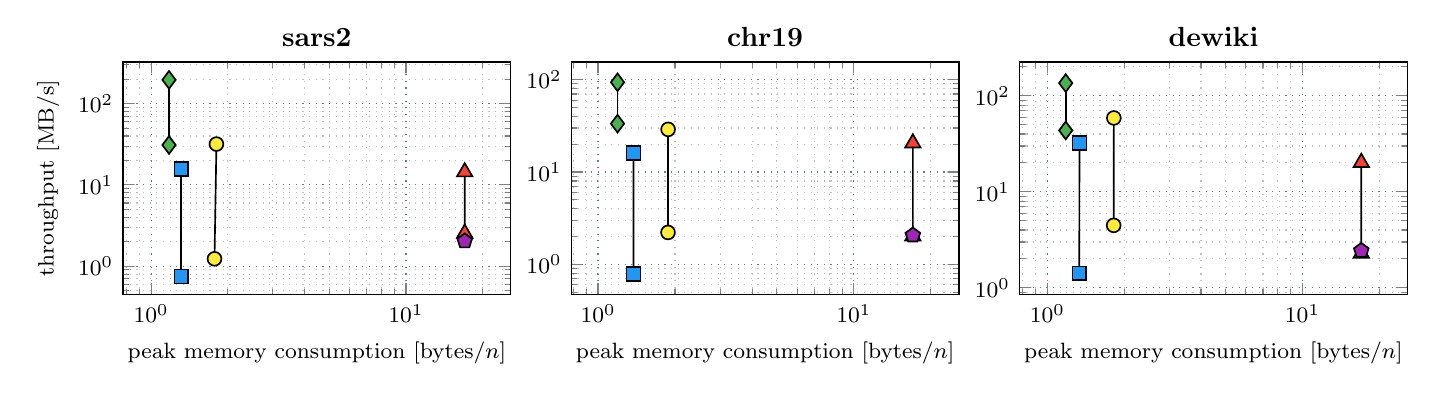
\begin{tikzpicture}[marks]
\begin{groupplot}[
    group style={group size=3 by 1, horizontal sep=22pt},
    throughput_style, xmode=log, ymode=log,
    width=140pt, height=84pt,
    xtick={0.01,0.1,1,10,100}, ytick={0.01,0.1,1,10,100,1000},
]

\nextgroupplot[
    title={sars2},
    xmin=0.7759, xmax=25.73, ymin=0.449, ymax=326,
    ylabel={throughput [MB/s]},
    xlabel={peak memory consumption [bytes/$n$]},
]

%% SELECT ((mem_peak + n)/(1.0*n)) AS x, throughput AS y
%% FROM results
%% WHERE text_name='sars2.50Gi' AND alg='lz77_sss' AND phr_mode=2 AND fact_mode=1 AND transf_mode=0
%% ORDER BY num_threads
\addplot[3_aprx] coordinates { (1.17445,30.9947) (1.17444,196.409) };

%% SELECT ((mem_peak + n)/(1.0*n)) AS x, throughput AS y
%% FROM results
%% WHERE text_name='sars2.50Gi' AND alg='lz77_sss' AND phr_mode=2 AND fact_mode=1 AND transf_mode=3
%% ORDER BY num_threads
\addplot[exact] coordinates { (1.31193,0.745169) (1.31193,15.6224) };

%% SELECT ((mem_peak + n)/(1.0*n)) AS x, throughput AS y
%% FROM results
%% WHERE text_name='sars2.50Gi' AND alg='lz77_sss' AND phr_mode=2 AND fact_mode=1 AND transf_mode=2
%% ORDER BY num_threads
\addplot[exact_smpl] coordinates { (1.77174,1.23195) (1.80272,31.827) };

%% SELECT ((mem_peak + n)/(1.0*n)) AS x, throughput AS y
%% FROM results
%% WHERE text_name='sars2.50Gi' AND alg='lpf'
%% ORDER BY num_threads
\addplot[lpf] coordinates { (17,2.54177) (17.0004,14.4456) };

%% SELECT ((mem_peak + n)/(1.0*n)) AS x, throughput AS y
%% FROM results
%% WHERE text_name='sars2.50Gi' AND alg='kkp2'
%% ORDER BY num_threads
\addplot[kkp2] coordinates { (17,2.03275) };

\annotatenear{1.17445,30.9947, -10pt, 5pt, 1.40}
\annotatenear{1.17444,196.409, 13pt, 0pt, 1.40}
\annotatenear{1.31193,0.745169, -11pt, 0pt, 1.00}
\annotatenear{1.31193,15.6224, -12pt, -4pt, 1.00}
\annotatenear{1.77174,1.23195, 0pt, -9pt, 1.00}
\annotatenear{1.80272,31.827, 3pt, 8pt, 1.00}
\annotatenear{17,2.54177, -8pt, 3pt, 1.00}
\annotatenear{17.0004,14.4456, 3pt, 8pt, 1.00}
\annotatenear{17,2.03275, -3pt, -8pt, 1.00}

\nextgroupplot[
    title={chr19},
    xmin=0.7874, xmax=25.73, ymin=0.4731, ymax=155.4,
    xlabel={peak memory consumption [bytes/$n$]},
]

%% SELECT (mem_peak/(1.0*n)) AS x, throughput AS y
%% FROM results
%% WHERE text_name='chr19.50Gi' AND alg='lz77_sss' AND phr_mode=2 AND fact_mode=1 AND transf_mode=0
%% ORDER BY num_threads
\addplot[3_aprx] coordinates { (1.19183,33.3941) (1.19183,93.6366) };

%% SELECT (mem_peak/(1.0*n)) AS x, throughput AS y
%% FROM results
%% WHERE text_name='chr19.50Gi' AND alg='lz77_sss' AND phr_mode=2 AND fact_mode=1 AND transf_mode=3
%% ORDER BY num_threads
\addplot[exact] coordinates { (1.37517,0.785167) (1.37658,16.0962) };

%% SELECT (mem_peak/(1.0*n)) AS x, throughput AS y
%% FROM results
%% WHERE text_name='chr19.50Gi' AND alg='lz77_sss' AND phr_mode=2 AND fact_mode=1 AND transf_mode=2
%% ORDER BY num_threads
\addplot[exact_smpl] coordinates { (1.87719,2.21895) (1.87864,28.9618) };

%% SELECT ((mem_peak + n)/(1.0*n)) AS x, throughput AS y
%% FROM results
%% WHERE text_name='chr19.50Gi' AND alg='lpf'
%% ORDER BY num_threads
\addplot[lpf] coordinates { (17,2.02384) (17.0004,20.5907) };

%% SELECT ((mem_peak + n)/(1.0*n)) AS x, throughput AS y
%% FROM results
%% WHERE text_name='chr19.50Gi' AND alg='kkp2'
%% ORDER BY num_threads
\addplot[kkp2] coordinates { (17,2.06581) };

\annotatenear{1.19183,33.3941, -8pt, -7pt, 2.02}
\annotatenear{1.19183,93.6366, 13pt, 0pt, 2.02}
\annotatenear{1.37517,0.785167, -11pt, 0pt, 1.00}
\annotatenear{1.37658,16.0962, -11pt, -7pt, 1.00}
\annotatenear{1.87719,2.21895, -2pt, -9pt, 1.00}
\annotatenear{1.87864,28.9618, 3pt, 8pt, 1.00}
\annotatenear{17,2.02384, 6pt, -10pt, 1.00}
\annotatenear{17.0004,20.5907, 3pt, 8pt, 1.00}
\annotatenear{17,2.06581, -8pt, -10pt, 1.00}

\nextgroupplot[
    title={dewiki},
    xmin=0.7796, xmax=25.73, ymin=0.8532, ymax=225.3,
    xlabel={peak memory consumption [bytes/$n$]},
]

%% SELECT (mem_peak/(1.0*n)) AS x, throughput AS y
%% FROM results
%% WHERE text_name='dewiki.50Gi' AND alg='lz77_sss' AND phr_mode=2 AND fact_mode=1 AND transf_mode=0
%% ORDER BY num_threads
\addplot[3_aprx] coordinates { (1.18002,43.6005) (1.18002,135.782) };

%% SELECT (mem_peak/(1.0*n)) AS x, throughput AS y
%% FROM results
%% WHERE text_name='dewiki.50Gi' AND alg='lz77_sss' AND phr_mode=2 AND fact_mode=1 AND transf_mode=3
%% ORDER BY num_threads
\addplot[exact] coordinates { (1.33332,1.41595) (1.3362,32.2297) };

%% SELECT (mem_peak/(1.0*n)) AS x, throughput AS y
%% FROM results
%% WHERE text_name='dewiki.50Gi' AND alg='lz77_sss' AND phr_mode=2 AND fact_mode=1 AND transf_mode=2
%% ORDER BY num_threads
\addplot[exact_smpl] coordinates { (1.81917,4.47431) (1.8221,58.8246) };

%% SELECT ((mem_peak + n)/(1.0*n)) AS x, throughput AS y
%% FROM results
%% WHERE text_name='dewiki.50Gi' AND alg='lpf'
%% ORDER BY num_threads
\addplot[lpf] coordinates { (17,2.29106) (17.0004,20.1883) };

%% SELECT ((mem_peak + n)/(1.0*n)) AS x, throughput AS y
%% FROM results
%% WHERE text_name='dewiki.50Gi' AND alg='kkp2'
%% ORDER BY num_threads
\addplot[kkp2] coordinates { (17,2.43683) };

\annotatenear{1.18002,43.6005, -10pt, 5pt, 1.44}
\annotatenear{1.18002,135.782, 13pt, 2pt, 1.44}
\annotatenear{1.33332,1.41595, 11pt, 0pt, 1.00}
\annotatenear{1.3362,32.2297, -10pt, -11pt, 1.00}
\annotatenear{1.81917,4.47431, -3pt, -8pt, 1.00}
\annotatenear{1.8221,58.8246, 13pt, 0pt, 1.00}
\annotatenear{17,2.29106, 0pt, -11pt, 1.00}
\annotatenear{17.0004,20.1883, 3pt, 8pt, 1.00}
\annotatenear{17,2.43683, -10pt, 8pt, 1.00}

\end{groupplot}
\end{tikzpicture}

\centering
\vspace*{0.15cm}
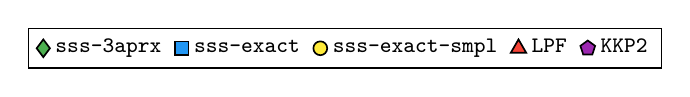
\begin{tikzpicture}[legendmarks]
\begin{axis}[legend,legend columns=5]

\addplot[3_aprx] coordinates { (0,0) };
\addlegendentry{\texttt{sss-3aprx}};
\addplot[exact] coordinates { (0,0) };
\addlegendentry{\texttt{sss-exact}};
\addplot[exact_smpl] coordinates { (0,0) };
\addlegendentry{\texttt{sss-exact-smpl}};
\addplot[lpf] coordinates { (0,0) };
\addlegendentry{\texttt{LPF}};
\addplot[kkp2] coordinates { (0,0) };
\addlegendentry{\texttt{KKP2}};

\end{axis}
\end{tikzpicture}
\vspace*{-0.1cm}
\caption{LZ77 factorization throughput versus peak memory consumption. Each point is annotated with the approximation ratio $z_{\mathrm{alg}}/z$.}
\label{fig:lz}

\end{figure*}

% ------------------------------- Figure 4 (fig:compress-decompress)
\begin{figure*}[t]
% IMPORT-DATA results results/results-zip.txt

\hspace*{-5pt}%
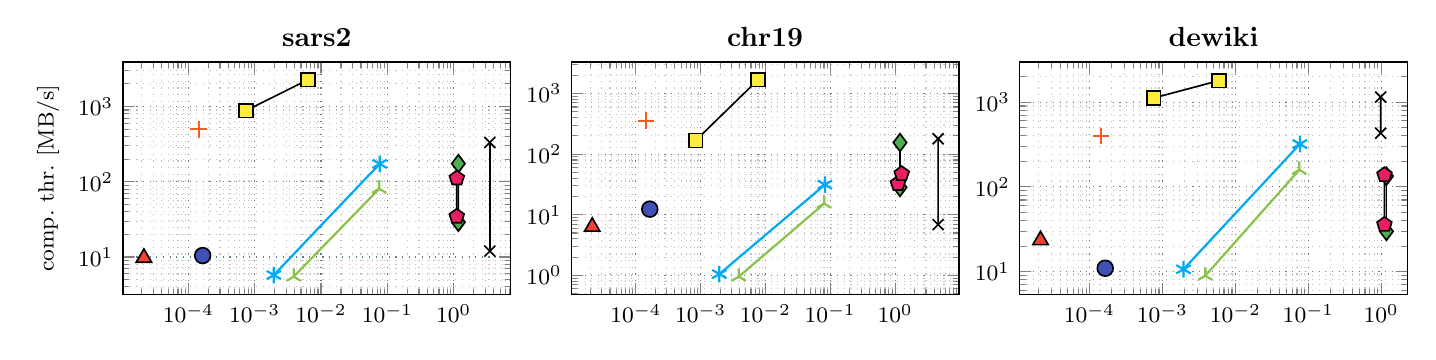
\begin{tikzpicture}[marks]
\begin{groupplot}[
    group style={group size=3 by 1, horizontal sep=22pt},
    throughput_style, xmode=log, ymode=log,
    width=140pt, height=84pt,
    ytick={0.1,1,10,100,1000,10000},
]

\nextgroupplot[
    title={sars2},
    xmin=1.043e-05, xmax=7.191, ymin=3.177, ymax=3918,
    ylabel={comp.\ thr.\ [MB/s]},
    xlabel={},
]

%% SELECT (mem_peak/(1.0*n)) AS x, throughput AS y
%% FROM results
%% WHERE text_name='sars2.50Gi' AND encoder='ssszip_bsc' AND type='compress'
%% ORDER BY num_threads
\addplot[ssszip_bsc] coordinates { (1.17445,28.9986) (1.17443,174.38) };

%% SELECT (mem_peak/(1.0*n)) AS x, throughput AS y
%% FROM results
%% WHERE text_name='sars2.50Gi' AND encoder='gzip' AND type='compress'
%% ORDER BY num_threads
\addplot[gzip] coordinates { (2.144e-05,9.75643) };

%% SELECT (mem_peak/(1.0*n)) AS x, throughput AS y
%% FROM results
%% WHERE text_name='sars2.50Gi' AND encoder='bzip2' AND type='compress'
%% ORDER BY num_threads
\addplot[bzip2] coordinates { (0.00016456,10.4455) };

%% SELECT (mem_peak/(1.0*n)) AS x, throughput AS y
%% FROM results
%% WHERE text_name='sars2.50Gi' AND encoder='xz' AND type='compress'
%% ORDER BY num_threads
\addplot[xz] coordinates { (0.00194744,5.75068) (0.0766994,173.296) };

%% SELECT (mem_peak/(1.0*n)) AS x, throughput AS y
%% FROM results
%% WHERE text_name='sars2.50Gi' AND encoder='lz4' AND type='compress'
%% ORDER BY num_threads
\addplot[lz4] coordinates { (0.000144,498.719) };

%% SELECT (mem_peak/(1.0*n)) AS x, throughput AS y
%% FROM results
%% WHERE text_name='sars2.50Gi' AND encoder='zstd' AND type='compress'
%% ORDER BY num_threads
\addplot[zstd] coordinates { (0.00073776,880.628) (0.00637016,2276.67) };

%% SELECT (mem_peak/(1.0*n)) AS x, throughput AS y
%% FROM results
%% WHERE text_name='sars2.50Gi' AND encoder='7z' AND type='compress'
%% ORDER BY num_threads
\addplot[7z] coordinates { (0.003874,5.4668) (0.0752062,80.6502) };

%% SELECT (mem_peak/(1.0*n)) AS x, throughput AS y
%% FROM results
%% WHERE text_name='sars2.50Gi' AND encoder='alz_8' AND type='compress'
%% ORDER BY num_threads
\addplot[alz_8] coordinates { (1.11094,34.5721) (1.11409,111.451) };

%% SELECT (mem_peak/(1.0*n)) AS x, throughput AS y
%% FROM results
%% WHERE text_name='sars2.50Gi' AND encoder='bsc_2047' AND type='compress'
%% ORDER BY num_threads
\addplot[bsc_2047] coordinates { (3.49951,11.9709) (3.49927,332.996) };

\annotatenear{1.17445,28.9986, -8pt, -7pt, 490}
\annotatenear{1.17443,174.38, 0pt, 9pt, 490}
\annotatenear{2.144e-05,9.75643, 3pt, 8pt, 5.75}
\annotatenear{0.00016456,10.4455, 3pt, 8pt, 18.4}
\annotatenear{0.00194744,5.75068, -3pt, 8pt, 244}
\annotatenear{0.0766994,173.296, 3pt, 8pt, 208}
\annotatenear{0.000144,498.719, 3pt, 8pt, 2.98}
\annotatenear{0.00073776,880.628, 0pt, 9pt, 55.6}
\annotatenear{0.00637016,2276.67, 0pt, -9pt, 55.6}
\annotatenear{0.003874,5.4668, 11pt, -2pt, 255}
\annotatenear{0.0752062,80.6502, 3pt, -8pt, 235}
\annotatenear{1.11094,34.5721, -10pt, 4pt, 614}
\annotatenear{1.11409,111.451, -11pt, 0pt, 614}
\annotatenear{3.49951,11.9709, -3pt, -8pt, 413}
\annotatenear{3.49927,332.996, 2pt, 9pt, 413}

\nextgroupplot[
    title={chr19},
    xmin=1.018e-05, xmax=9.655, ymin=0.485, ymax=3312,
    xlabel={},
]

%% SELECT (mem_peak/(1.0*n)) AS x, throughput AS y
%% FROM results
%% WHERE text_name='chr19.50Gi' AND encoder='ssszip_bsc' AND type='compress'
%% ORDER BY num_threads
\addplot[ssszip_bsc] coordinates { (1.19183,28.2124) (1.19183,155.297) };

%% SELECT (mem_peak/(1.0*n)) AS x, throughput AS y
%% FROM results
%% WHERE text_name='chr19.50Gi' AND encoder='gzip' AND type='compress'
%% ORDER BY num_threads
\addplot[gzip] coordinates { (2.128e-05,6.34436) };

%% SELECT (mem_peak/(1.0*n)) AS x, throughput AS y
%% FROM results
%% WHERE text_name='chr19.50Gi' AND encoder='bzip2' AND type='compress'
%% ORDER BY num_threads
\addplot[bzip2] coordinates { (0.00016448,12.387) };

%% SELECT (mem_peak/(1.0*n)) AS x, throughput AS y
%% FROM results
%% WHERE text_name='chr19.50Gi' AND encoder='xz' AND type='compress'
%% ORDER BY num_threads
\addplot[xz] coordinates { (0.00194712,1.05123) (0.082741,31.3711) };

%% SELECT (mem_peak/(1.0*n)) AS x, throughput AS y
%% FROM results
%% WHERE text_name='chr19.50Gi' AND encoder='lz4' AND type='compress'
%% ORDER BY num_threads
\addplot[lz4] coordinates { (0.000144,355.041) };

%% SELECT (mem_peak/(1.0*n)) AS x, throughput AS y
%% FROM results
%% WHERE text_name='chr19.50Gi' AND encoder='zstd' AND type='compress'
%% ORDER BY num_threads
\addplot[zstd] coordinates { (0.00084048,167.869) (0.00770056,1689.17) };

%% SELECT (mem_peak/(1.0*n)) AS x, throughput AS y
%% FROM results
%% WHERE text_name='chr19.50Gi' AND encoder='7z' AND type='compress'
%% ORDER BY num_threads
\addplot[7z] coordinates { (0.00387408,0.951095) (0.0805718,15.2577) };

%% SELECT (mem_peak/(1.0*n)) AS x, throughput AS y
%% FROM results
%% WHERE text_name='chr19.50Gi' AND encoder='alz_8' AND type='compress'
%% ORDER BY num_threads
\addplot[alz_8] coordinates { (1.10759,32.5531) (1.26674,47.2694) };

%% SELECT (mem_peak/(1.0*n)) AS x, throughput AS y
%% FROM results
%% WHERE text_name='chr19.50Gi' AND encoder='bsc_2047' AND type='compress'
%% ORDER BY num_threads
\addplot[bsc_2047] coordinates { (4.61909,6.87248) (4.61883,179.245) };

\annotatenear{1.19183,28.2124, -4pt, -10pt, 441}
\annotatenear{1.19183,155.297, 2pt, 9pt, 441}
\annotatenear{2.128e-05,6.34436, 3pt, 8pt, 3.65}
\annotatenear{0.00016448,12.387, 3pt, 8pt, 4.08}
\annotatenear{0.00194712,1.05123, -2pt, 11pt, 4.67}
\annotatenear{0.082741,31.3711, 3pt, 8pt, 4.64}
\annotatenear{0.000144,355.041, 3pt, 8pt, 1.92}
\annotatenear{0.00084048,167.869, -3pt, -8pt, 3.53}
\annotatenear{0.00770056,1689.17, 2pt, -11pt, 3.53}
\annotatenear{0.00387408,0.951095, 13pt, -2pt, 4.65}
\annotatenear{0.0805718,15.2577, 2pt, -11pt, 4.64}
\annotatenear{1.10759,32.5531, -11pt, 0pt, 386}
\annotatenear{1.26674,47.2694, 11pt, 0pt, 386}
\annotatenear{4.61909,6.87248, -3pt, -8pt, 15.7}
\annotatenear{4.61883,179.245, 0pt, 9pt, 15.7}

\nextgroupplot[
    title={dewiki},
    xmin=1.109e-05, xmax=2.272, ymin=5.384, ymax=2978,
    xlabel={},
]

%% SELECT (mem_peak/(1.0*n)) AS x, throughput AS y
%% FROM results
%% WHERE text_name='dewiki.50Gi' AND encoder='ssszip_bsc' AND type='compress'
%% ORDER BY num_threads
\addplot[ssszip_bsc] coordinates { (1.18002,29.8432) (1.18001,133.624) };

%% SELECT (mem_peak/(1.0*n)) AS x, throughput AS y
%% FROM results
%% WHERE text_name='dewiki.50Gi' AND encoder='gzip' AND type='compress'
%% ORDER BY num_threads
\addplot[gzip] coordinates { (2.136e-05,23.5029) };

%% SELECT (mem_peak/(1.0*n)) AS x, throughput AS y
%% FROM results
%% WHERE text_name='dewiki.50Gi' AND encoder='bzip2' AND type='compress'
%% ORDER BY num_threads
\addplot[bzip2] coordinates { (0.00016448,10.9694) };

%% SELECT (mem_peak/(1.0*n)) AS x, throughput AS y
%% FROM results
%% WHERE text_name='dewiki.50Gi' AND encoder='xz' AND type='compress'
%% ORDER BY num_threads
\addplot[xz] coordinates { (0.0019472,10.6628) (0.0767607,320.299) };

%% SELECT (mem_peak/(1.0*n)) AS x, throughput AS y
%% FROM results
%% WHERE text_name='dewiki.50Gi' AND encoder='lz4' AND type='compress'
%% ORDER BY num_threads
\addplot[lz4] coordinates { (0.000144,400.306) };

%% SELECT (mem_peak/(1.0*n)) AS x, throughput AS y
%% FROM results
%% WHERE text_name='dewiki.50Gi' AND encoder='zstd' AND type='compress'
%% ORDER BY num_threads
\addplot[zstd] coordinates { (0.00075856,1118.37) (0.00596008,1794.16) };

%% SELECT (mem_peak/(1.0*n)) AS x, throughput AS y
%% FROM results
%% WHERE text_name='dewiki.50Gi' AND encoder='7z' AND type='compress'
%% ORDER BY num_threads
\addplot[7z] coordinates { (0.00387408,8.93557) (0.0752878,158.841) };

%% SELECT (mem_peak/(1.0*n)) AS x, throughput AS y
%% FROM results
%% WHERE text_name='dewiki.50Gi' AND encoder='alz_8' AND type='compress'
%% ORDER BY num_threads
\addplot[alz_8] coordinates { (1.10656,35.8879) (1.10913,138.591) };

%% SELECT (mem_peak/(1.0*n)) AS x, throughput AS y
%% FROM results
%% WHERE text_name='dewiki.50Gi' AND encoder='bsc_2047' AND type='compress'
%% ORDER BY num_threads
\addplot[bsc_2047] coordinates { (0.984135,430.147) (0.984448,1147.33) };

\annotatenear{1.18002,29.8432, -8pt, -7pt, 490}
\annotatenear{1.18001,133.624, -13pt, -2pt, 490}
\annotatenear{2.136e-05,23.5029, 3pt, 8pt, 3.32}
\annotatenear{0.00016448,10.9694, 3pt, 8pt, 14.9}
\annotatenear{0.0019472,10.6628, -3pt, 8pt, 391}
\annotatenear{0.0767607,320.299, 3pt, 8pt, 251}
\annotatenear{0.000144,400.306, 3pt, 8pt, 2.48}
\annotatenear{0.00075856,1118.37, 3pt, 8pt, 106}
\annotatenear{0.00596008,1794.16, -3pt, -8pt, 106}
\annotatenear{0.00387408,8.93557, 11pt, 0pt, 364}
\annotatenear{0.0752878,158.841, 2pt, -11pt, 304}
\annotatenear{1.10656,35.8879, -10pt, 5pt, 526}
\annotatenear{1.10913,138.591, -10pt, 5pt, 526}
\annotatenear{0.984135,430.147, -10pt, 4pt, 461}
\annotatenear{0.984448,1147.33, 3pt, 8pt, 461}

\end{groupplot}
\end{tikzpicture}

\hspace*{-5pt}%
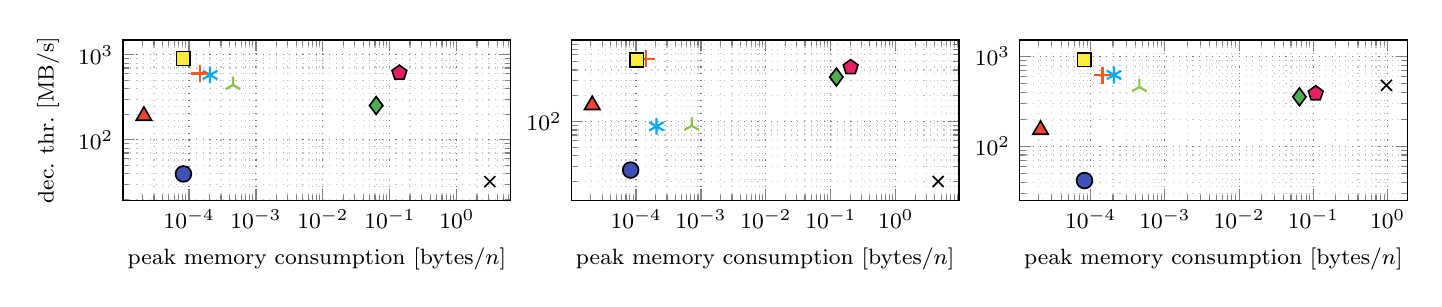
\begin{tikzpicture}[marks]
\begin{groupplot}[
    group style={group size=3 by 1, horizontal sep=22pt},
    throughput_style, xmode=log, ymode=log,
    width=140pt, height=58pt,
    ytick={0.1,1,10,100,1000,10000},
]

\nextgroupplot[
    xmin=1.038e-05, xmax=6.357, ymin=19.4, ymax=1501,
    ylabel={dec.\ thr.\ [MB/s]},
    xlabel={peak memory consumption [bytes/$n$]},
]

%% SELECT (mem_peak/(1.0*n)) AS x, throughput AS y
%% FROM results
%% WHERE text_name LIKE 'sars2.50Gi%' AND encoder='ssszip_bsc' AND type='decompress'
\addplot[ssszip_bsc] coordinates { (0.0624046,253.332) };

%% SELECT (mem_peak/(1.0*n)) AS x, throughput AS y
%% FROM results
%% WHERE text_name LIKE 'sars2.50Gi%' AND encoder='gzip' AND type='decompress'
\addplot[gzip] coordinates { (2.12e-05,191.359) };

%% SELECT (mem_peak/(1.0*n)) AS x, throughput AS y
%% FROM results
%% WHERE text_name LIKE 'sars2.50Gi%' AND encoder='bzip2' AND type='decompress'
\addplot[bzip2] coordinates { (8.264e-05,39.6943) };

%% SELECT (mem_peak/(1.0*n)) AS x, throughput AS y
%% FROM results
%% WHERE text_name LIKE 'sars2.50Gi%' AND encoder='xz' AND type='decompress'
\addplot[xz] coordinates { (0.00020648,580.064) };

%% SELECT (mem_peak/(1.0*n)) AS x, throughput AS y
%% FROM results
%% WHERE text_name LIKE 'sars2.50Gi%' AND encoder='lz4' AND type='decompress'
\addplot[lz4] coordinates { (0.00014408,604.074) };

%% SELECT (mem_peak/(1.0*n)) AS x, throughput AS y
%% FROM results
%% WHERE text_name LIKE 'sars2.50Gi%' AND encoder='zstd' AND type='decompress'
\addplot[zstd] coordinates { (8.208e-05,904.648) };

%% SELECT (mem_peak/(1.0*n)) AS x, throughput AS y
%% FROM results
%% WHERE text_name LIKE 'sars2.50Gi%' AND encoder='7z' AND type='decompress'
\addplot[7z] coordinates { (0.00045384,442.903) };

%% SELECT (mem_peak/(1.0*n)) AS x, throughput AS y
%% FROM results
%% WHERE text_name LIKE 'sars2.50Gi%' AND encoder='alz_8' AND type='decompress'
\addplot[alz_8] coordinates { (0.138878,613.107) };

%% SELECT (mem_peak/(1.0*n)) AS x, throughput AS y
%% FROM results
%% WHERE text_name LIKE 'sars2.50Gi%' AND encoder='bsc_2047' AND type='decompress'
\addplot[bsc_2047] coordinates { (3.11346,32.2027) };

\annotatenear{0.0624046,253.332, -3pt, 8pt, 490}
\annotatenear{2.12e-05,191.359, 0pt, 9pt, 5.75}
\annotatenear{8.264e-05,39.6943, 3pt, 8pt, 18.4}
\annotatenear{0.00020648,580.064, 6pt, 10pt, 244}
\annotatenear{0.00014408,604.074, -6pt, -10pt, 2.98}
\annotatenear{8.208e-05,904.648, -13pt, 2pt, 55.6}
\annotatenear{0.00045384,442.903, -3pt, -8pt, 255}
\annotatenear{0.138878,613.107, 3pt, -8pt, 614}
\annotatenear{3.11346,32.2027, 2pt, 9pt, 413}

\nextgroupplot[
    xmin=1.012e-05, xmax=9.383, ymin=12.14, ymax=896.6,
    xlabel={peak memory consumption [bytes/$n$]},
]

%% SELECT (mem_peak/(1.0*n)) AS x, throughput AS y
%% FROM results
%% WHERE text_name LIKE 'chr19.50Gi%' AND encoder='ssszip_bsc' AND type='decompress'
\addplot[ssszip_bsc] coordinates { (0.121676,330.728) };

%% SELECT (mem_peak/(1.0*n)) AS x, throughput AS y
%% FROM results
%% WHERE text_name LIKE 'chr19.50Gi%' AND encoder='gzip' AND type='decompress'
\addplot[gzip] coordinates { (2.112e-05,156.143) };

%% SELECT (mem_peak/(1.0*n)) AS x, throughput AS y
%% FROM results
%% WHERE text_name LIKE 'chr19.50Gi%' AND encoder='bzip2' AND type='decompress'
\addplot[bzip2] coordinates { (8.256e-05,27.3226) };

%% SELECT (mem_peak/(1.0*n)) AS x, throughput AS y
%% FROM results
%% WHERE text_name LIKE 'chr19.50Gi%' AND encoder='xz' AND type='decompress'
\addplot[xz] coordinates { (0.00020624,88.3222) };

%% SELECT (mem_peak/(1.0*n)) AS x, throughput AS y
%% FROM results
%% WHERE text_name LIKE 'chr19.50Gi%' AND encoder='lz4' AND type='decompress'
\addplot[lz4] coordinates { (0.000144,540.28) };

%% SELECT (mem_peak/(1.0*n)) AS x, throughput AS y
%% FROM results
%% WHERE text_name LIKE 'chr19.50Gi%' AND encoder='zstd' AND type='decompress'
\addplot[zstd] coordinates { (0.00010248,520.749) };

%% SELECT (mem_peak/(1.0*n)) AS x, throughput AS y
%% FROM results
%% WHERE text_name LIKE 'chr19.50Gi%' AND encoder='7z' AND type='decompress'
\addplot[7z] coordinates { (0.00072008,89.6062) };

%% SELECT (mem_peak/(1.0*n)) AS x, throughput AS y
%% FROM results
%% WHERE text_name LIKE 'chr19.50Gi%' AND encoder='alz_8' AND type='decompress'
\addplot[alz_8] coordinates { (0.202066,429.313) };

%% SELECT (mem_peak/(1.0*n)) AS x, throughput AS y
%% FROM results
%% WHERE text_name LIKE 'chr19.50Gi%' AND encoder='bsc_2047' AND type='decompress'
\addplot[bsc_2047] coordinates { (4.49449,20.1393) };

\annotatenear{0.121676,330.728, -3pt, -8pt, 441}
\annotatenear{2.112e-05,156.143, 3pt, 8pt, 3.65}
\annotatenear{8.256e-05,27.3226, -2pt, 9pt, 4.08}
\annotatenear{0.00020624,88.3222, 3pt, -8pt, 4.67}
\annotatenear{0.000144,540.28, 6pt, -10pt, 1.92}
\annotatenear{0.00010248,520.749, -11pt, 2pt, 3.53}
\annotatenear{0.00072008,89.6062, 3pt, 8pt, 4.65}
\annotatenear{0.202066,429.313, 11pt, 0pt, 386}
\annotatenear{4.49449,20.1393, 0pt, 9pt, 15.7}

\nextgroupplot[
    xmin=1.109e-05, xmax=1.841, ymin=25.09, ymax=1525,
    xlabel={peak memory consumption [bytes/$n$]},
]

%% SELECT (mem_peak/(1.0*n)) AS x, throughput AS y
%% FROM results
%% WHERE text_name LIKE 'dewiki.50Gi%' AND encoder='ssszip_bsc' AND type='decompress'
\addplot[ssszip_bsc] coordinates { (0.0649919,354.853) };

%% SELECT (mem_peak/(1.0*n)) AS x, throughput AS y
%% FROM results
%% WHERE text_name LIKE 'dewiki.50Gi%' AND encoder='gzip' AND type='decompress'
\addplot[gzip] coordinates { (2.112e-05,152.502) };

%% SELECT (mem_peak/(1.0*n)) AS x, throughput AS y
%% FROM results
%% WHERE text_name LIKE 'dewiki.50Gi%' AND encoder='bzip2' AND type='decompress'
\addplot[bzip2] coordinates { (8.256e-05,41.6419) };

%% SELECT (mem_peak/(1.0*n)) AS x, throughput AS y
%% FROM results
%% WHERE text_name LIKE 'dewiki.50Gi%' AND encoder='xz' AND type='decompress'
\addplot[xz] coordinates { (0.0002064,620.969) };

%% SELECT (mem_peak/(1.0*n)) AS x, throughput AS y
%% FROM results
%% WHERE text_name LIKE 'dewiki.50Gi%' AND encoder='lz4' AND type='decompress'
\addplot[lz4] coordinates { (0.000144,616.731) };

%% SELECT (mem_peak/(1.0*n)) AS x, throughput AS y
%% FROM results
%% WHERE text_name LIKE 'dewiki.50Gi%' AND encoder='zstd' AND type='decompress'
\addplot[zstd] coordinates { (8.2e-05,918.609) };

%% SELECT (mem_peak/(1.0*n)) AS x, throughput AS y
%% FROM results
%% WHERE text_name LIKE 'dewiki.50Gi%' AND encoder='7z' AND type='decompress'
\addplot[7z] coordinates { (0.00045344,455.774) };

%% SELECT (mem_peak/(1.0*n)) AS x, throughput AS y
%% FROM results
%% WHERE text_name LIKE 'dewiki.50Gi%' AND encoder='alz_8' AND type='decompress'
\addplot[alz_8] coordinates { (0.107712,386.333) };

%% SELECT (mem_peak/(1.0*n)) AS x, throughput AS y
%% FROM results
%% WHERE text_name LIKE 'dewiki.50Gi%' AND encoder='bsc_2047' AND type='decompress'
\addplot[bsc_2047] coordinates { (0.967083,476.11) };

\annotatenear{0.0649919,354.853, -3pt, 8pt, 490}
\annotatenear{2.112e-05,152.502, 3pt, 8pt, 3.32}
\annotatenear{8.256e-05,41.6419, 3pt, 8pt, 14.9}
\annotatenear{0.0002064,620.969, 2pt, 9pt, 391}
\annotatenear{0.000144,616.731, -3pt, -8pt, 2.48}
\annotatenear{8.2e-05,918.609, -11pt, 2pt, 106}
\annotatenear{0.00045344,455.774, -3pt, -8pt, 364}
\annotatenear{0.107712,386.333, 3pt, 8pt, 526}
\annotatenear{0.967083,476.11, 2pt, 9pt, 461}

\end{groupplot}
\end{tikzpicture}

\centering
\vspace*{0.15cm}
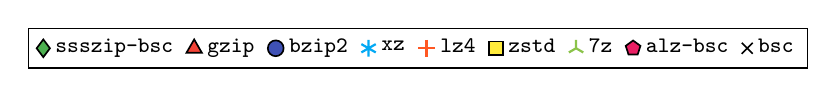
\begin{tikzpicture}[legendmarks]
\begin{axis}[legend,legend columns=10]

\addplot[ssszip_bsc] coordinates { (0,0) };
\addlegendentry{\texttt{ssszip-bsc}};
\addplot[gzip] coordinates { (0,0) };
\addlegendentry{\texttt{gzip}};
\addplot[bzip2] coordinates { (0,0) };
\addlegendentry{\texttt{bzip2}};
\addplot[xz] coordinates { (0,0) };
\addlegendentry{\texttt{xz}};
\addplot[lz4] coordinates { (0,0) };
\addlegendentry{\texttt{lz4}};
\addplot[zstd] coordinates { (0,0) };
\addlegendentry{\texttt{zstd}};
\addplot[7z] coordinates { (0,0) };
\addlegendentry{\texttt{7z}};
\addplot[alz_8] coordinates { (0,0) };
\addlegendentry{\texttt{alz-bsc}};
\addplot[bsc_2047] coordinates { (0,0) };
\addlegendentry{\texttt{bsc}};

\end{axis}
\end{tikzpicture}
\vspace*{-0.1cm}
\caption{Compression and decompression throughput versus peak memory consumption. The top row shows compression, the bottom row decompression.}
\label{fig:compress-decompress}

\end{figure*}

\end{document}
